%%%%%%%%%%%%%%%%%%%%%%%%%%%%%%%%%%%%%%%%%%%%%%%%%%%%%%%%%%%%%%%%%%%%%%%%%%%%%%%
%                                                                             %
% Anwendungsbeispiel für das Beamer-Template TU Chemnitz                      %
% (c) Mario Haustein (mario.haustein@hrz.tu-chemnitz.de), 2013-2014           %
%                                                                             %
%%%%%%%%%%%%%%%%%%%%%%%%%%%%%%%%%%%%%%%%%%%%%%%%%%%%%%%%%%%%%%%%%%%%%%%%%%%%%%%

\usepackage{ifxetex}
\usepackage{ifluatex}
\ifxetex
\usepackage[babelshorthands]{polyglossia}
\setmainlanguage{german}
\else\ifluatex
\usepackage[babelshorthands]{polyglossia}
\setmainlanguage{german}
\else
\usepackage[utf8]{inputenc}
\usepackage[ngerman]{babel}
\fi\fi
\usepackage{url}
\usepackage{tikz}
\usepackage{amsmath}
\usepackage{exscale}
\usepackage{listings}
\usepackage{listingsutf8}
\usepackage{textcomp}
\usepackage{chemfig}
\usepackage{metalogo}
\usepackage{tabularx}
\usepackage{subfigure}


\renewcommand{\arraystretch}{1.2}
% Trennstellen für URLs
\def\UrlBreaks{\do\:\do\.\do\@\do\\\do\/\do\!\do\_\do\|\do\;\do\>\do\]%
 \do\)\do\,\do\?\do\'\do+\do\=\do\#}
\def\UrlBigBreaks{}

% Voreinstellungen für Quellcodelistings
\lstset{basicstyle=\ttfamily,keywordstyle=\fontfamily{lmss}\bfseries,breaklines,tabsize=2}
\ifxetex\else\ifluatex\else\lstset{inputencoding=utf8/latin1}\fi\fi
\lstdefinestyle{block}{basicstyle=\ttfamily,keywordstyle=\fontfamily{lmss}\bfseries,breakindent=10pt}
\lstdefinestyle{numberedblock}{basicstyle=\ttfamily,keywordstyle=\fontfamily{lmss}\bfseries,numbers=left,numberstyle=\scriptsize,xleftmargin=20pt,frame=leftline,breakindent=10pt}

% TUC-Templates laden.
\usetheme[fakcolor=if]{tuc2014}
\mode<article>{\usepackage{beamerarticletuc2014}}


% Metadaten
\title{Kolloquium zur Bachelorarbeit}
\subtitle[Interaktive, grafische Steuerung des Growing Neural Gas]{Interaktive, grafische Steuerung des Growing Neural Gas}
\author{Tobias Gall}
\date[\today]{\today}
\institute[TUC, IF]{TU Chemnitz, Fakultät für Informatik}
\titlegraphic{\includegraphics[height=0.2\textheight]{tuc2014/logo/tuc_green}}
\tucurl{http://www.tu-chemnitz.de/}


\begin{document}
\begingroup
\tucthreeheadlines
\frame{\titlepage}
\endgroup


\frame{
	\frametitle{Gliederung}
	\tableofcontents{}
}

\section{Zielsetzung}
\begingroup
\vspace*{\fill}
\centerline{\Large\textbf{Aufgabenstellung}}

\bigskip
\bigskip

\begin{quote}
\begin{center}
\Large
Interaktive grafische Steuerung des Growing Neural Gas
\end{center}
\end{quote}

\bigskip

In dieser Bachelorarbeit soll ein Konzept zu interaktiven, grafikbasierten Steuerung des Growing Neural
Gas (GNG) erarbeitet und prototypisch umgesetzt werden. Der Anwender soll die einzelnen
Arbeitsschritte (Trainingsphasen) des GNG anhand einer zweidimensionalen grafischen Darstellung des
neuronalen Netzes nachvollziehen können. Die Steuerung soll Einstellmöglichkeiten für Parameter des
GNG bieten.
\vspace*{\fill}
\endgroup

\section{Growing Neural Gas}
\begin{frame}
	\frametitle{Growing Neural Gas}
	\begin{itemize}
		\item künstliches neuronales Netz
		\item 1995 von Bernd Fritzke entwickelt
		\item lernt selbstständig seine Struktur
	\end{itemize}
	\begin{figure}[h!]
		\centering
		
\includegraphics[width=0.7\textwidth]{bilder/animated_training-26.png}
		\caption{Simulation Growing Neural Gas}
		\label{fig:simulation}
	\end{figure}
\end{frame}
\note{\begin{enumerate}
	\item Initialize the set with two units
	\item Generate at random an input signal $\xi$ according to $p(\xi)$
	\item Determine the winner $s_{1}$ and the second-nearest unit $s_{2}$
	\item If a connection between does not exist already, create it. Set the age of the connection to zero
	\item Add the squared distance between the input signal and the winner to a local error variable
	\item Adapt the reference vectors of the winner and its direct topological neighbors by fractions $epsilon_{winner}$ and $epsilon_{neighbor}$, respectively, of the total distance to the input signal
	\item Increment the age of all edges emanating from winner $s_{1}$
	\item Remove edges with an age larger than $age_{max}$. If this results in units having no more emanating edges, remove those units as well
\end{enumerate}}
\note{\begin{enumerate}
	\setcounter{enumi}{8}
	\item If the number of input signals generated so far is an integer multiple of a parameter $\lambda$, insert a new unit as follows
	\begin{enumerate}
		\item Determine the unit $q$ with the maximum accumulated error
		\item Determine among the neighbors of $q$ the unit $f$ with the maximum accumulated error
		\item Add a new unit r to the network and interpolate its reference vector from $q$ and $f$
		\item Insert edges connecting the new unit $r$ with units $q$ and $f$, and remove the original edge between $q$ and $f$
		\item Decrease the error variables of $q$ and $f$ by a fraction $\alpha$
		\item Interpolate the error variable of $r$ from $q$ and $f$
	\end{enumerate}
	\item Decrease the error variables of all units by a fraction $\beta$
	\item If a stopping criterion (e.g., net size or some performance measure) is not yet fulfilled continue with step 2
\end{enumerate}}

\section{Anforderungen}
\begin{frame}
    \begin{center}
        \Huge{Anforderungen}
    \end{center}
\end{frame}
\begin{frame}
    \frametitle{Übersicht}
    \begin{figure}[h]
        \centering
        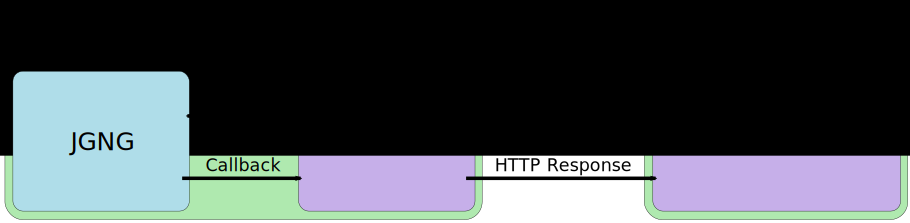
\includegraphics[width=\textwidth]{../figures/client-server.pdf}
        \caption{Übersicht Komponenten}
    \end{figure}
\end{frame}
\begin{frame}
    \frametitle{Anforderungen an die API}
    \begin{itemize}
        \item Auswahl des Algorithmus, zum Trainieren des neuronalen Netzes
        \item Einstellung aller Parameter des Algorithmus
        \item Auswahl eines Datensatzes, zum Trainieren des neuronalen Netzes
        \item Festlegung der Anzahl an Durchläufen für eine Trainingseinheit
        \item Bereitstellung der topologischen Daten des neuronalen Netzes, die der Algorithmus generiert hat
        \item Paralleles Trainieren mehrerer neuronaler Netze
    \end{itemize}
\end{frame}
\begin{frame}
    \frametitle{Anforderungen an die Webanwendung}
    \begin{itemize}
        \item Nutzung der Funktionalität der API
        \item Übersichtliche Darstellung des Trainingsprozesses des neuronalen Netzes
        \item Benutzerfreundliche Möglichkeit zur Parametrisierung des Algorithmus
    \end{itemize}
\end{frame}

\section{Implementierung}
\subsection*{REST API}
\begin{frame}
    \begin{center}
        \Huge{REST API}
    \end{center}
    \begin{figure}[h]
        \centering
        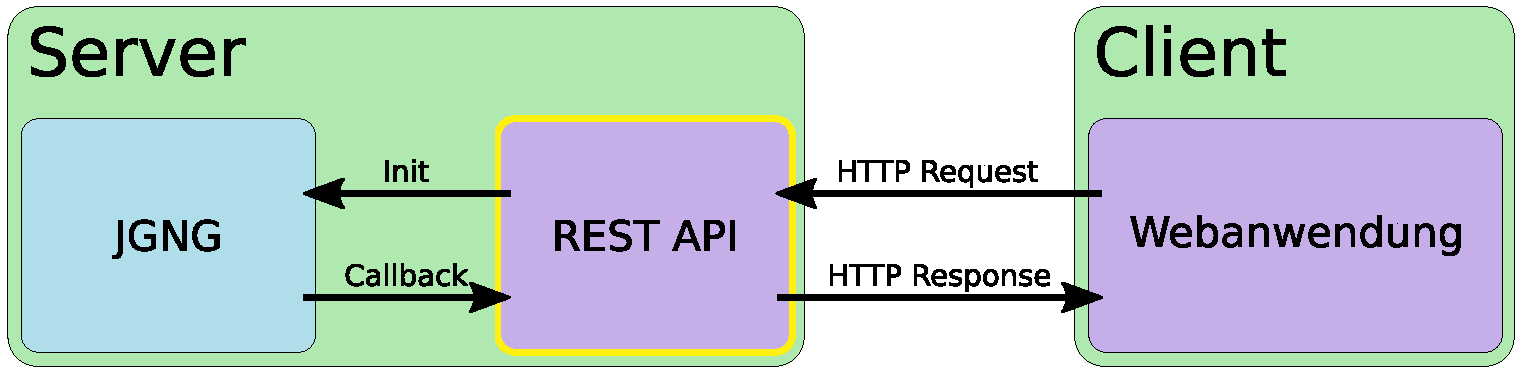
\includegraphics[width=\textwidth]{bilder/client-server_rest-active.pdf}
    \end{figure}
\end{frame}
\subsubsection*{Usecasediagramm API}
\begin{frame}
    \begin{figure}[h]
        \centering
        \includegraphics[width=0.6\textwidth]{../figures/apicontroller.pdf}
        \caption{Usecasediagramm API}
    \end{figure}
\end{frame}
%\subsection*{URL Struktur}
%\begin{frame}
%    \frametitle{URL Struktur}
%    \begin{center}
%        \begin{tabularx}{\textwidth}{ lll }
%            \textbf{HTTP-Methode} & \textbf{Pfad} & \textbf{Methode im Controller} \\
%            \hline
%            POST & \texttt{/training} & setTraining \\
%            POST & \texttt{/training/<id>} & setTrainingID \\
%            GET & \texttt{/training} & getTrainings \\
%            GET & \texttt{/training/<id>} & getTraining \\
%            PUT & \texttt{/training/<id>} & setSettings \\
%            DELETE & \texttt{/training/<id>} & deleteTraining \\
%            POST & \texttt{/train/<id>} & setTrain \\
%            GET & \texttt{/train/<id>} & getTrain
%        \end{tabularx}
%    \end{center}
%\end{frame}
\subsubsection*{Umsetzung}
\begin{frame}
    \frametitle{Aspekte der Implementierung}
    \begin{itemize}
        \item Initalisierung des JGNG
        \item Implementierung des Delegationsinterfaces(Callback)
        \item Datenstruktur für Neuronen und Kanten
        \item Verarbeiten der Nutzeranfragen und Bereitstellung der Daten
    \end{itemize}
\end{frame}
\begin{frame}
    \frametitle{JGNG Callback}
    \begin{figure}[h]
        \centering
        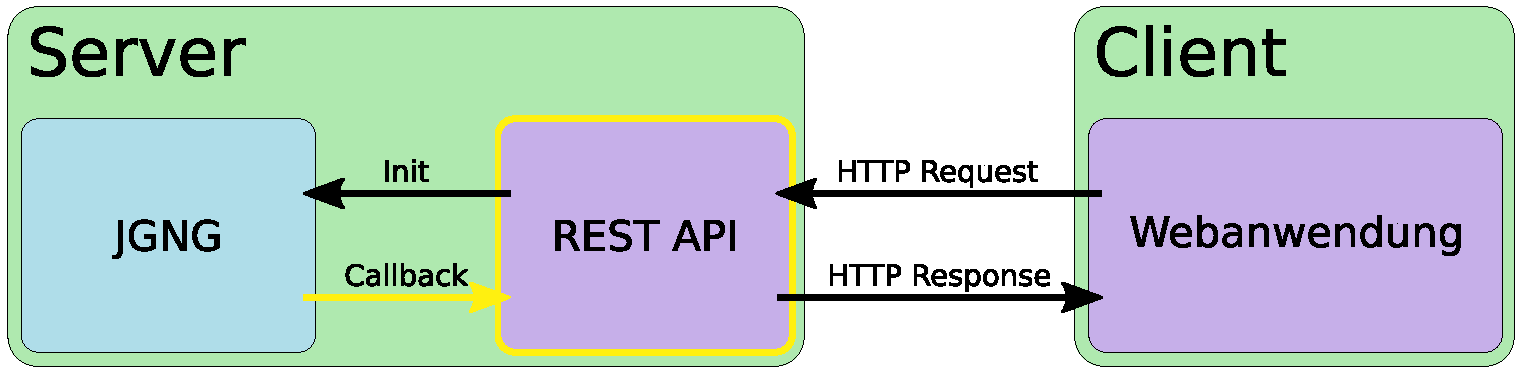
\includegraphics[width=\textwidth]{bilder/client-server_callback-active.pdf}
    \end{figure}
    \begin{itemize}
        \item Callback wird als Interface vom Algorithmus bereitgestellt und von der REST API impementiert
        \item Er empfängt alle Änderungen am neuronalem Netz
        \item \textbf{Problem:} NeuronenID sind nur Listindizes
        \newline $\rightarrow$ Mapping auf eindeutige IDs durch atomare Zählvariable
        \item Speicherung der Neuronen und Kanten
    \end{itemize}
\end{frame}
%\begin{frame}
%    \begin{figure}[h]
%        \centering
%        \includegraphics[width=\textwidth]{../figures/gngcallback.pdf}
%        \caption{Kommunikationsdiagramm GNGCallback}
%    \end{figure}
%\end{frame}
\begin{frame}
    \frametitle{Datenstruktur}
    \begin{itemize}
        \item Speicherung der Neuronen und Kanten als Objekte
        \newline $\rightarrow$ Verknüpfung mit zusätzlichen Attributen
        \item Zusammenfassung der Neuronen und Kanten in zwei verschiedenen Objekten
    \end{itemize}
    \begin{figure}[h]
        \centering
        \includegraphics[width=\textwidth]{../figures/datenstruktur.pdf}
        \caption{Klassendiagramm Datenstruktur}
    \end{figure}
\end{frame}
\begin{frame}
    \frametitle{Verwaltung der Anfragen}
    \begin{figure}[h]
        \centering
        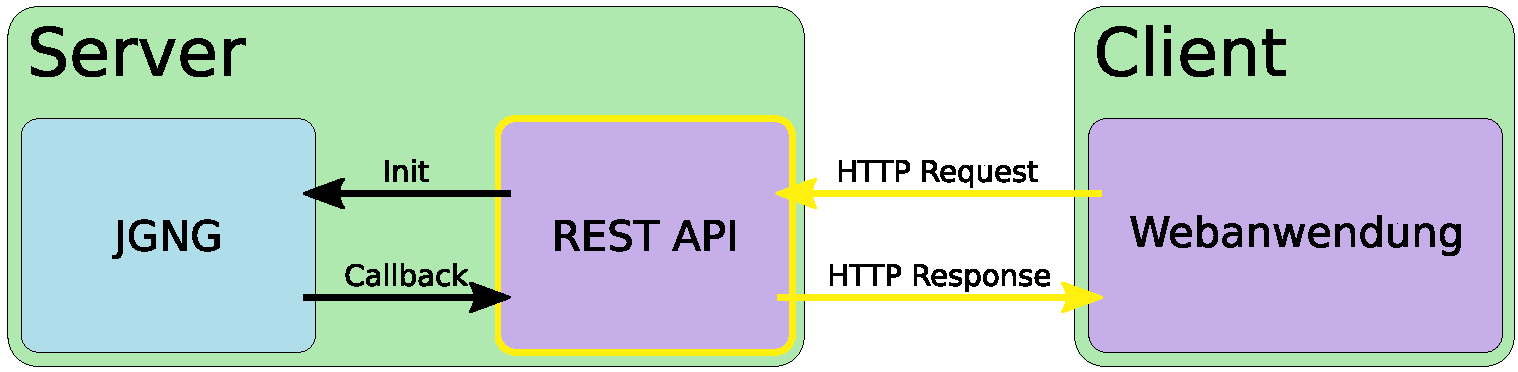
\includegraphics[width=\textwidth]{bilder/client-server_http-active.pdf}
    \end{figure}
    %\begin{center}
    %    \begin{footnotesize}
    %        \begin{tabularx}{\textwidth}{ lll }
    %            \textbf{HTTP-Methode} & \textbf{Pfad} & \textbf{Methode im Controller} \\
    %            \hline
    %            POST & \texttt{/training} & setTraining \\
    %            GET & \texttt{/training/<id>} & getTraining \\
    %            ... & &
    %        \end{tabularx}
    %    \end{footnotesize}
    %\end{center}
\end{frame}
\begin{frame}
    \frametitle{Einsatz des Spring Boot Framework}
    \begin{figure}[h]
        \centering
        \includegraphics[width=\textwidth]{../figures/springboot.pdf}
        %\caption{Spring Boot Framework}
    \end{figure}
\end{frame}
\begin{frame}
    \frametitle{REST Controller}
    Der REST Controller übernimmt folgende Aufgaben:
    \begin{itemize}
        \item Initialisierung des JGNG
        \begin{itemize}
            \item Kapselung des JGNG in einem Wrapper mit eindeutiger ID
            \newline $\rightarrow$ mehrere JGNG parallel verfügbar
            \item Übergabe eines Callback und Datenhaltung
        \end{itemize}
        \item Entgegennehmen der Einstellungen für das JGNG
        \item Zurückgeben des neuronalen Netzes
        \item Zurückgeben einer Trainingseinheit
    \end{itemize}
    Optional:
    \begin{itemize}
        \item Auflisten aller neuronalen Netze
        \item Löschen eines neuronalen Netzes
    \end{itemize}
\end{frame}

\subsection*{Webanwendung}
\begin{frame}
    \begin{center}
        \Huge{Webanwendung}
    \end{center}
    \begin{figure}[h]
        \centering
        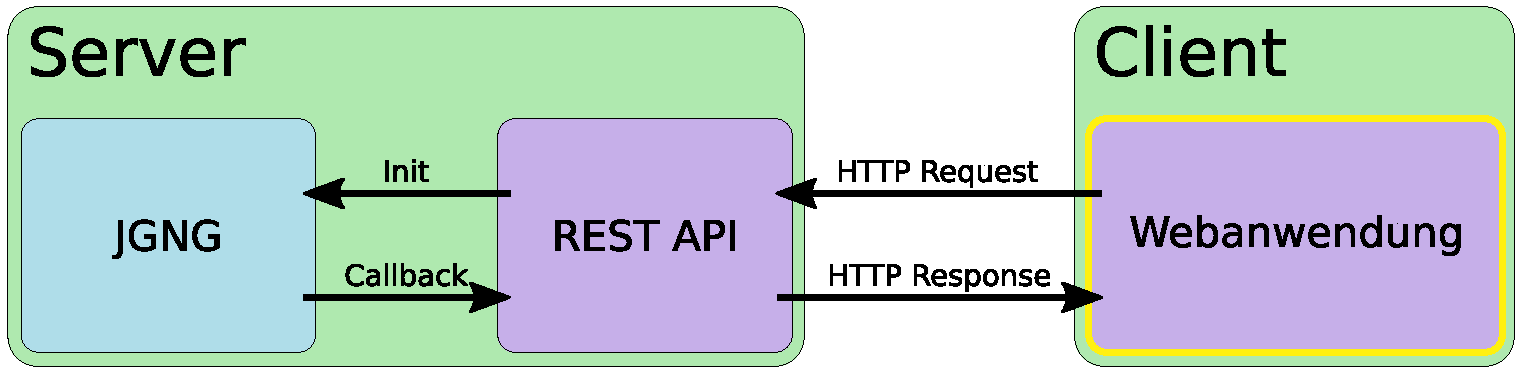
\includegraphics[width=\textwidth]{bilder/client-server_web-active.pdf}
    \end{figure}
\end{frame}
\subsubsection*{Layout und Umsetzung}
\begin{frame}
    \frametitle{Layout und Umsetzung}
    \begin{itemize}
        \item fixiertes Layout in der Aufteilung von 75\% (Graph) zu 25\% (Einstellungen) der Breite des Fensters
        \item Verwendung von \textbf{Bootstrap} (CSS) für die grundlegende Gestaltung
        \item Verwendung von \textbf{jQuery} (JS) zur Kommunikation mit der API mittels AJAX und JSON
        \item Verwendung des \textbf{Sigma} (JS) für die Darstellung des Graphen
    \end{itemize}
\end{frame}
\begin{frame}
    \frametitle{Ergebnis}
    \begin{figure}[h]
        \centering
        \includegraphics[width=0.9\textwidth]{../figures/jgng_net.png}
        %\caption{Webanwendung mit trainiertem JGNG}
    \end{figure}
\end{frame}


%\section{Zusammenfassung}
%

\section*{}
\begin{frame}
	\begin{center}
        \Huge{Vielen Dank.}
	\end{center}
\end{frame}

\end{document}
